\documentclass[11pt,a4paper]{article}
\usepackage[T1]{fontenc}
\usepackage{lmodern}
\usepackage[top=0.30in, bottom=0.30in, left=0.68in, right=0.68in, headheight=0pt, headsep=0pt]{geometry}
\usepackage{amsmath,amssymb}
\usepackage{xcolor}
\usepackage{tikz}
\usetikzlibrary{arrows.meta,positioning,calc,decorations.pathreplacing}
\usepackage{tcolorbox}
\usepackage{hyperref}
\usepackage{booktabs}
\usepackage{caption}

\hypersetup{
    colorlinks=true,
    linkcolor=blue!70!black,
    citecolor=blue!70!black,
    urlcolor=blue!70!black
}

% Custom Callout Boxes matching house style
\newtcolorbox{learningobj}{
    colback=blue!3!white,
    colframe=blue!60!black,
    fonttitle=\bfseries\sffamily,
    fontupper=\small,
    title={$\blacktriangleright$ LEARNING OBJECTIVE},
    arc=1.2mm,
    boxrule=0.7pt,
    left=2.5mm, right=2.5mm, top=0.5mm, bottom=0.5mm,
    before skip=0.2mm, after skip=0.5mm
}

\newtcolorbox{groundbreaking}{
    colback=teal!4!white,
    colframe=teal!60!black,
    fonttitle=\bfseries\sffamily,
    fontupper=\small,
    title={$\bigstar$ GROUNDBREAKING FINDING},
    arc=1.2mm,
    boxrule=0.7pt,
    left=2.5mm, right=2.5mm, top=0.3mm, bottom=0.3mm,
    before skip=0.1mm, after skip=0.3mm
}

\newtcolorbox{physicalinsight}{
    colback=yellow!6!white,
    colframe=orange!75!black,
    fonttitle=\bfseries\sffamily,
    fontupper=\small,
    title={$\blacktriangleright$ PHYSICAL INSIGHT},
    arc=1.2mm,
    boxrule=0.7pt,
    left=2.5mm, right=2.5mm, top=0.4mm, bottom=0.4mm,
    before skip=0.2mm, after skip=0.4mm
}

\setlength{\parindent}{0pt}
\setlength{\parskip}{1.2pt}

\newcommand{\diagsec}[1]{\vspace{1.6pt}\textbf{\large #1}\vspace{0.5pt}\par}

\begin{document}
\setlength{\abovedisplayskip}{1.0pt}
\setlength{\belowdisplayskip}{1.0pt}

% ==================== PAGE 1 ====================
\subsection*{1.5 Diagnostic Failure Modes: Stress-Testing Silicon and Acoustic Boundaries}

\begin{learningobj}
Rather than treating the 16~kHz / 25~ms / $N=512$ / dense Mel stack as sacred, this section breaks each knob and shows where silicon and speech physics refuse to follow.
\end{learningobj}

\textbf{Organic Bridge from Section 1.4: Testing Physical Limits at the Hardware Boundary.} In Section~1.4, we grounded the front-end DSP pipeline in physical silicon, demonstrating that the streaming time-domain buffer occupies exactly $1{,}600\text{ B}$ of memory and the uncompressed Mel filterbank requires $80 \times 257 \times 4\text{ B} = 82{,}240\text{ B}$. Most critically, the isolation finding proved that front-end feature extraction runs entirely on-chip within fixed memory boundaries, isolated from external bus contention and guaranteed to satisfy the $10\text{ ms}$ real-time hop cadence.

However, an algorithm that runs smoothly under nominal parameters often conceals sharp mathematical and physical failure boundaries. When a systems engineer attempts to optimize performance by turning architectural knobs---such as tripling the sampling rate for higher fidelity, slashing the window duration to cut latency, omitting zero-padding to reduce FFT points, or storing filter matrices in dense floating-point format---the underlying physics of acoustic wave propagation and spatial silicon microarchitectures violently push back. The four diagnostic scenarios below examine these boundary conditions.

\diagsec{Diagnostic Scenario 1: The Sampling Rate Illusion}

\textbf{The Naive Hypothesis.} A systems engineer proposes upgrading the front-end audio acquisition pipeline from the standard $f_s = 16\text{ kHz}$ to the professional studio sampling standard $f_s = 48\text{ kHz}$. The stated engineering rationale is that tripling the temporal sampling rate will preserve subtle high-frequency acoustic nuances, suppress quantization noise, and boost keyword-spotting accuracy, while keeping the acoustic window length at $25\text{ ms}$ and the hop cadence at $10\text{ ms}$.

\textbf{Worked Mathematical Breakdown.}

\textbf{1.~Sample Counts ($L_{48}$ and $H_{48}$):} At $f_s = 48\text{ kHz}$, the sampling period shrinks to $T_s = 1 / 48{,}000\text{ s} \approx 20.833\ \mu\text{s}$. To preserve the physical frame duration of $25\text{ ms}$ and hop cadence of $10\text{ ms}$, the required sample counts scale linearly:
\begin{equation}
  L_{48} = 48{,}000 \times 0.025 = 1{,}200\text{ samples}, \qquad H_{48} = 48{,}000 \times 0.010 = 480\text{ samples}
\end{equation}
Both quantities exactly triple compared to the nominal $16\text{ kHz}$ baseline ($L = 400$, $H = 160$).

\textbf{2.~On-Chip Memory Allocation:} Storing $1{,}200$ samples in 32-bit single-precision floating point (FP32, 4~bytes/sample) requires $1{,}200 \times 4\text{ B} = 4{,}800\text{ bytes}$. A single physical 36-kbit Block RAM (RAMB36E2) on the AMD XCK26 MPSoC provides exactly $36{,}864\text{ bits} = 4{,}608\text{ bytes}$ of storage. Because $4{,}800\text{ bytes} > 4{,}608\text{ bytes}$, the circular buffer overflows a single physical BRAM primitive. The synthesis engine is forced to allocate \textbf{two dedicated 36-kbit Block RAM blocks}, doubling the silicon memory footprint.

\textbf{3.~Acoustic Reality and Nyquist Bounds:} Under Nyquist-Shannon sampling, $f_s = 48\text{ kHz}$ captures frequencies up to $24\text{ kHz}$. However, the vocal tract resonances that define human speech---the fundamental pitch ($F_0 \approx 85\text{--}255\text{ Hz}$) and vowel formants ($F_1\text{--}F_4$ spanning $250\text{--}4{,}500\text{ Hz}$), as well as sibilant fricatives ($/s/, /\int/$ peaking between $4{,}000\text{--}7{,}500\text{ Hz}$)---are entirely contained below $8\text{ kHz}$. The expanded $8\text{--}24\text{ kHz}$ octaves contain only ambient thermal hiss and circuit switching noise. Transforming $1{,}200$ samples forces downstream FFT length to at least $N = 2{,}048$, more than quadrupling butterfly compute. The system incurs a $3\times$ memory penalty, $3\times$ I/O throughput, and $>4\times$ DSP operations for \textbf{identically zero keyword-spotting gain}.

\begin{physicalinsight}
Tripling the sampling rate from $16\text{ kHz}$ to $48\text{ kHz}$ overflows the $4{,}608\text{-byte}$ boundary of a physical 36-kbit Block RAM block and quadruples downstream arithmetic, squandering silicon area and dynamic power to capture ultrasonic frequencies outside the biomechanical limits of human vocal cords.
\end{physicalinsight}

\clearpage
% ==================== PAGE 2 ====================
\diagsec{Diagnostic Scenario 2: The Gabor--Heisenberg Penalty}

\textbf{The Naive Hypothesis.} To eliminate speech processing lag in an ultra-responsive edge voice assistant, an embedded designer seeks to aggressively reduce the physical frame accumulation floor. Rather than waiting $25\text{ ms}$ for $400$ audio samples to accumulate, the designer cuts the analysis window length by $80\%$, setting $L = 80$ samples ($\Delta t = 5\text{ ms}$) at $f_s = 16\text{ kHz}$, arguing that modern deep neural networks can extract acoustic features just as easily from shorter time slices.

\textbf{Worked Mathematical Breakdown.}

\textbf{1.~Time-Frequency Localization Limits:} The theoretical floor of time-frequency localization is bounded by the Gabor--Heisenberg uncertainty relation $\Delta t \cdot \Delta f \ge 1 / (4\pi)$. This sets an immutable Heisenberg floor of $\Delta f_{\text{min}} \approx 3.2\text{ Hz}$ at $\Delta t = 25\text{ ms}$, and $\approx 16\text{ Hz}$ at $\Delta t = 5\text{ ms}$. In practical spectral analysis with discrete windows, however, resolving power is determined by the Rayleigh spectral main-lobe width $\Delta f \approx 1/T$: at $25\text{ ms}$, the Rayleigh width is $\Delta f_{25} = 1/0.025\text{ s} = 40\text{ Hz}$ (with a Hamming null-to-null bandwidth of $4/T = 160\text{ Hz}$, or rectangular null-to-null of $2/T = 80\text{ Hz}$). When the window is truncated to $5\text{ ms}$, the Rayleigh width broadens to $\Delta f_5 = 1/0.005\text{ s} = 200\text{ Hz}$ (with a Hamming null-to-null bandwidth of $4/T = 800\text{ Hz}$, or rectangular null-to-null of $2/T = 400\text{ Hz}$).

\textbf{2.~Formant Smearing and Phonetic Collapse:} In human vowel production, adjacent formants---specifically the first two formants ($F_1$ and $F_2$), which distinguish vowel identities---frequently lie within $150\text{--}200\text{ Hz}$ of each other. When the filter main lobe broadens to $\Delta f \approx 200\text{ Hz}$ (with Hamming nulls spanning $800\text{ Hz}$), the spectral analyzer can no longer resolve two distinct spectral peaks spaced $180\text{ Hz}$ apart. The two distinct formants blur together into a single broad, merged spectral mass. Acoustic distinctions between cardinal vowels collapse---for example, the close front vowel $/i/$ (high $F_2$, low $F_1$) merges indistinguishably with the close back vowel $/u/$ (compact low $F_1, F_2$), destroying the phonetic representations required by downstream acoustic models.

\textbf{3.~Biomechanical Incompatibility:} The human vocal apparatus is constrained by physical inertia: the tongue, velum, jaw, and pharyngeal muscles cannot physically change state in under $20\text{--}30\text{ ms}$. More critically, $5\text{ ms}$ is significantly shorter than the fundamental pitch period of a typical low adult male voice ($1 / 85\text{ Hz} \approx 11.8\text{ ms}$). A $5\text{ ms}$ window captures only an incomplete fraction of a single glottal cycle. Depending on whether the $5\text{ ms}$ window coincides with the open or closed glottal phase, the extracted spectral energy swings erratically by tens of decibels from frame to frame, causing severe feature instability.

\begin{physicalinsight}
Cutting the window length below $20\text{ ms}$ does not create an ultra-low-latency voice engine; it constructs a low-resolution spectral blur. Temporal latency cannot be reduced past the biomechanical inertia of the human vocal tract without violating the Gabor--Heisenberg bound and fusing critical formant frequencies.
\end{physicalinsight}

\diagsec{Diagnostic Scenario 3: The Discrete Transform Trap}

\textbf{The Naive Hypothesis.} A hardware architect inspecting the STFT pipeline notices that after windowing, the audio frame contains exactly $L = 400$ samples. Rather than appending $112$ artificial zeros to reach a power-of-two size ($N = 512$), the architect argues that the FPGA should compute a direct 400-point Discrete Fourier Transform (DFT), avoiding the memory overhead of storing zeros and eliminating what appears to be superfluous computation.

\textbf{Worked Mathematical Breakdown.}

\textbf{1.~Direct DFT Complexity:} Evaluating $201$ independent frequency bins ($k = 0, \dots, 200$) from $400$ samples via $X[k] = \sum_{n=0}^{L-1} x[n] e^{-j 2\pi k n / L}$ requires $L = 400$ complex multiply-accumulate operations per bin:
$\text{Workload}_{\text{DFT}} = 201 \times 400 = 80{,}400\text{ complex MACs / frame}$.

\textbf{2.~Radix-2 Cooley-Tukey FFT Complexity:} Appending $112$ zeros to form a length-$512$ vector ($N = 2^9$) unlocks the radix-2 Cooley-Tukey FFT, bounded by $(N/2) \log_2 N$ butterfly stages:
$\text{Workload}_{\text{FFT}} = \frac{512}{2} \log_2(512) = 256 \times 9 = 2{,}304\text{ butterfly operations / frame}$.

\textbf{3.~Silicon Hardware Cost Comparison:} Comparing workloads yields $\text{Reduction Ratio} = 80{,}400 / 2{,}304 \approx 34.9\times$. On an FPGA, an $\mathcal{O}(L^2)$ direct DFT within the $10\text{ ms}$ deadline requires dedicating hundreds of DSP48E2 slices or overclocking multipliers, exhausting routing channels and power. Conversely, the radix-2 FFT maps into an unrolled cascade consuming fewer than a dozen DSPs. The $112$ padded zeros cost exactly zero arithmetic operations, inject zero synthetic distortion, and unlock a \textbf{$34.9\times$ silicon savings}.

\begin{physicalinsight}
Zero-padding is not arithmetic waste; it is an architectural enabler. Padded zeros cost zero multiply-accumulate operations while unlocking power-of-two recursive symmetry that slashes silicon compute by $34.9\times$.
\end{physicalinsight}

\clearpage
% ==================== PAGE 3 ====================
\diagsec{Diagnostic Scenario 4: The Dense Matrix Bottleneck}

\textbf{The Naive Hypothesis.} A software-trained engineer maps the Mel filterbank stage onto the FPGA by treating the filterbank weights as a standard dense matrix. The stage multiplies $K = 257$ spectral energy bins by $M = 80$ triangular filter vectors: $E_\ell[m] = \sum_{k=0}^{256} g_m[k] P_\ell[k]$. Storing this transformation as a dense FP32 matrix requires $80 \times 257 \times 4\text{ B} = 82{,}240\text{ bytes} = 80.3\text{ KiB}$, which consumes $82{,}240 / 4{,}608 \approx 18$ physical 36-kbit Block RAM blocks ($12.5\%$ of total on-chip BRAM on the Kria KV260).

\textbf{Worked Mathematical Breakdown.}

\textbf{1.~Filterbank Sparsity Exploitation:} Because each Mel filter $g_m[k]$ is a compact triangle non-zero only between $[k_{m-1}, k_{m+1}]$, adjacent filters overlap by $50\%$. Each frequency bin $k$ is covered by at most two filters. Out of $80 \times 257 = 20{,}560$ matrix elements, only a tiny fraction are non-zero:
$\text{Non-Zero Weights} \approx 2 \times 257 \approx 514$ (or $80 \times 6.4 \approx 512$ active weights). Over $97.5\%$ of the dense matrix consists of structural zeros.

\textbf{2.~Compressed Sparse Storage Formulation:} Compressing each filter into quantized 16-bit integer coefficients (INT16, 2~bytes per weight) requires $514 \times 2 = 1{,}028\text{ B}$. Storing metadata $(k_{\text{min}}, K_m)$ for 80 bands ($1\text{ byte}$ each, $80 \times 2 = 160\text{ B}$) yields a total compressed memory footprint of:
$\text{Compressed Memory} = 1{,}028\text{ B} + 160\text{ B} = 1{,}188\text{ bytes}$.

\textbf{3.~Silicon Resource and Bandwidth Impact:} Comparing dense FP32 against sparse INT16 reveals:
$\text{BRAM Footprint} = 1{,}188\text{ B} / 4{,}608\text{ B} \approx 25.8\% \text{ of 1 BRAM}$, with $\text{Reduction Ratio} = 82{,}240\text{ B} / 1{,}188\text{ B} \approx 69.2\times$. Sparse compression collapses the Mel filterbank memory footprint from $18$ BRAM blocks down to $25.8\%$ of a single BRAM, immediately liberating $17$ physical BRAM primitives ($17 \times 4{,}608\text{ B} = 78{,}336\text{ B} \approx 76.5\text{ KiB}$) for neural network acoustic weights. Furthermore, memory read bandwidth collapses from $20{,}560$ reads down to just $514$ reads per frame---\textbf{a $40\times$ reduction in memory access operations}.

\begin{physicalinsight}
Storing structural zeros in physical memory is architectural suicide. Sparse triangular compression collapses the Mel filterbank footprint by $69.2\times$, compressing 18 Block RAMs into a quarter of a single primitive and slashing memory read bandwidth by $40\times$.
\end{physicalinsight}

\noindent\begin{minipage}{\textwidth}
\centering
\resizebox{0.92\textwidth}{!}{% Figure 1.5a: Four-Knob Silicon and Acoustic Damage Board
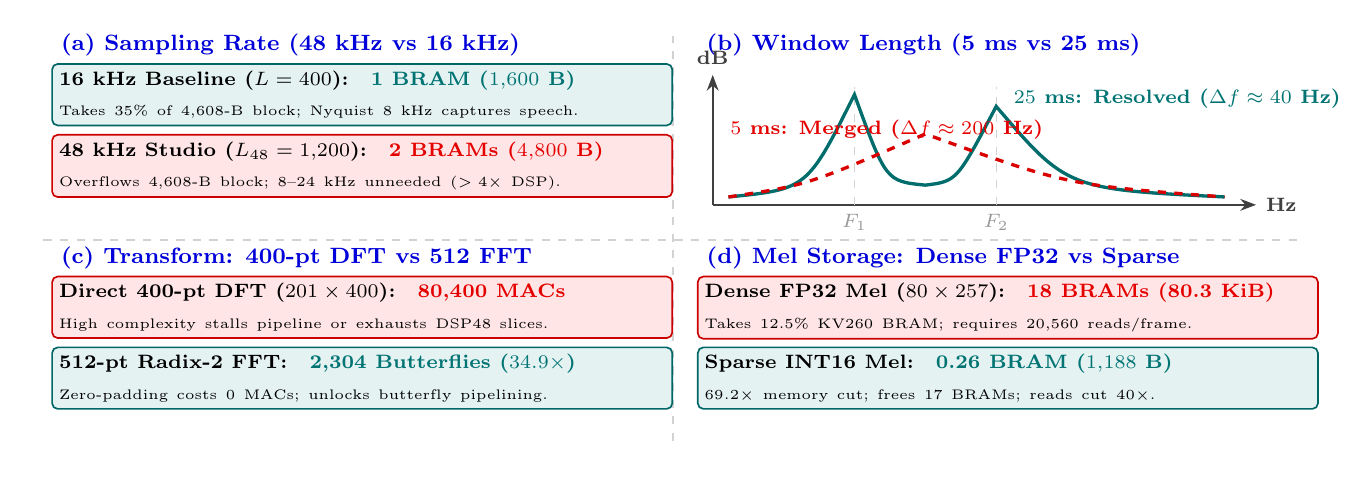
\begin{tikzpicture}[
  >=Stealth,
  font=\small
]

\useasboundingbox (0, 0) rectangle (16.4, 5.4);

% Dashed dividers
\draw[gray!35, thick, dashed] (8.2, 0.15) -- (8.2, 5.30);
\draw[gray!35, thick, dashed] (0.2, 2.70) -- (16.2, 2.70);

% ==================== PANEL (a): Top-Left: Sampling Rate Overflow ====================
\begin{scope}[xshift=0.2cm, yshift=2.70cm]
  \node[font=\bfseries\footnotesize, text=blue!85!black, anchor=west] at (0.1, 2.48) 
    {(a) Sampling Rate (48 kHz vs 16 kHz)};

  % 16 kHz Baseline Box
  \node[draw=teal!80!black, fill=teal!10, rounded corners=2pt, semithick, text width=7.7cm, inner sep=2.5pt, align=left, anchor=north west] 
    at (0.1, 2.25) {
    \scriptsize\textbf{16 kHz Baseline ($L=400$):}\quad \textcolor{teal!90!black}{\textbf{1 BRAM ($1{,}600\text{ B}$)}}\\
    \tiny Takes $35\%$ of 4,608-B block; Nyquist $8\text{ kHz}$ captures speech.
  };

  % 48 kHz Studio Box
  \node[draw=red!80!black, fill=red!10, rounded corners=2pt, semithick, text width=7.7cm, inner sep=2.5pt, align=left, anchor=north west] 
    at (0.1, 1.35) {
    \scriptsize\textbf{48 kHz Studio ($L_{48}=1{,}200$):}\quad \textcolor{red!90!black}{\textbf{2 BRAMs ($4{,}800\text{ B}$)}}\\
    \tiny Overflows 4,608-B block; $8\text{--}24\text{ kHz}$ unneeded ($>4\times$ DSP).
  };
\end{scope}

% ==================== PANEL (b): Top-Right: Gabor-Heisenberg Smear ====================
\begin{scope}[xshift=8.4cm, yshift=2.70cm]
  \node[font=\bfseries\footnotesize, text=blue!85!black, anchor=west] at (0.1, 2.48) 
    {(b) Window Length (5 ms vs 25 ms)};

  % Mini spectral plot
  \draw[->, black!75, semithick] (0.3, 0.45) -- (7.2, 0.45) node[right, font=\scriptsize\bfseries] {Hz};
  \draw[->, black!75, semithick] (0.3, 0.45) -- (0.3, 2.10) node[above, font=\scriptsize\bfseries] {dB};

  % Formant grid lines
  \draw[gray!35, thin, dashed] (2.1, 0.45) -- (2.1, 1.95);
  \node[below, font=\scriptsize, text=gray!80] at (2.1, 0.45) {$F_1$};
  \draw[gray!35, thin, dashed] (3.9, 0.45) -- (3.9, 1.95);
  \node[below, font=\scriptsize, text=gray!80] at (3.9, 0.45) {$F_2$};

  % 25 ms curve (sharp twin peaks, teal)
  \draw[teal!85!black, very thick] 
    (0.5, 0.55) .. controls (1.5, 0.65) .. (2.1, 1.85) 
    .. controls (2.5, 0.75) .. (3.0, 0.70) 
    .. controls (3.4, 0.75) .. (3.9, 1.70) 
    .. controls (4.8, 0.65) .. (6.8, 0.55);
  \node[font=\scriptsize\bfseries, text=teal!90!black, anchor=west] at (4.0, 1.80) {
    $25\text{ ms}$: Resolved ($\Delta f \approx 40\text{ Hz}$)
  };

  % 5 ms curve (single smeared blob, red dashed)
  \draw[red!85!black, very thick, dashed] 
    (0.5, 0.55) .. controls (1.5, 0.70) .. (3.0, 1.35) 
    .. controls (4.8, 0.70) .. (6.8, 0.55);
  \node[font=\scriptsize\bfseries, text=red!90!black, anchor=west] at (0.4, 1.40) {
    $5\text{ ms}$: Merged ($\Delta f \approx 200\text{ Hz}$)
  };
\end{scope}

% ==================== PANEL (c): Bottom-Left: Transform Workload ====================
\begin{scope}[xshift=0.2cm, yshift=0.0cm]
  \node[font=\bfseries\footnotesize, text=blue!85!black, anchor=west] at (0.1, 2.48) 
    {(c) Transform: 400-pt DFT vs 512 FFT};

  % Direct DFT Box
  \node[draw=red!80!black, fill=red!10, rounded corners=2pt, semithick, text width=7.7cm, inner sep=2.5pt, align=left, anchor=north west] 
    at (0.1, 2.25) {
    \scriptsize\textbf{Direct 400-pt DFT ($201 \times 400$):}\quad \textcolor{red!90!black}{\textbf{80,400 MACs}}\\
    \tiny High complexity stalls pipeline or exhausts DSP48 slices.
  };

  % Radix-2 FFT Box
  \node[draw=teal!80!black, fill=teal!10, rounded corners=2pt, semithick, text width=7.7cm, inner sep=2.5pt, align=left, anchor=north west] 
    at (0.1, 1.35) {
    \scriptsize\textbf{512-pt Radix-2 FFT:}\quad \textcolor{teal!90!black}{\textbf{2,304 Butterflies ($34.9\times$)}}\\
    \tiny Zero-padding costs 0 MACs; unlocks butterfly pipelining.
  };
\end{scope}

% ==================== PANEL (d): Bottom-Right: Dense vs Sparse Mel Memory ====================
\begin{scope}[xshift=8.4cm, yshift=0.0cm]
  \node[font=\bfseries\footnotesize, text=blue!85!black, anchor=west] at (0.1, 2.48) 
    {(d) Mel Storage: Dense FP32 vs Sparse};

  % Dense BRAM Box
  \node[draw=red!80!black, fill=red!10, rounded corners=2pt, semithick, text width=7.7cm, inner sep=2.5pt, align=left, anchor=north west] 
    at (0.1, 2.25) {
    \scriptsize\textbf{Dense FP32 Mel ($80 \times 257$):}\quad \textcolor{red!90!black}{\textbf{18 BRAMs (80.3 KiB)}}\\
    \tiny Takes 12.5\% KV260 BRAM; requires 20,560 reads/frame.
  };

  % Sparse INT16 Box
  \node[draw=teal!80!black, fill=teal!10, rounded corners=2pt, semithick, text width=7.7cm, inner sep=2.5pt, align=left, anchor=north west] 
    at (0.1, 1.35) {
    \scriptsize\textbf{Sparse INT16 Mel:}\quad \textcolor{teal!90!black}{\textbf{0.26 BRAM ($1{,}188\text{ B}$)}}\\
    \tiny $69.2\times$ memory cut; frees 17 BRAMs; reads cut $40\times$.
  };
\end{scope}

\end{tikzpicture}
}\\[2pt]
{\scriptsize\textbf{Figure 1.5a}: \textbf{The four-knob silicon and acoustic damage board.} (1)~\textbf{What it is:} Diagnostic failure modes across the streaming front-end when deviating from nominal parameters. (2)~\textbf{What to look at:} In (a), $48\text{ kHz}$ sampling overflows a single 36-kbit BRAM ($4{,}800\text{ B} > 4{,}608\text{ B}$), forcing two BRAM blocks. In (b), shortening the window to $5\text{ ms}$ broadens spectral main lobe to $200\text{ Hz}$, merging adjacent formants $F_1$ and $F_2$. In (c), a direct 400-point DFT requires $80{,}400$ complex MACs, whereas zero-padding to $512$ points unlocks the radix-2 FFT at $2{,}304$ butterflies ($34.9\times$ reduction). In (d), sparse INT16 compression collapses Mel filter storage from $80.3\text{ KiB}$ ($18$ BRAMs) to $1{,}188\text{ B}$ ($25.8\%$ of one BRAM), a $69.2\times$ memory reduction. (3)~\textbf{What it proves:} Standard front-end parameters are Pareto-optimal compromises dictated by acoustic physics and FPGA microarchitecture.\par}
\end{minipage}

\begin{groundbreaking}
The standard front-end pipeline parameters---$16\text{ kHz}$ sampling, $25\text{ ms}$ windowing, $N=512$ zero-padding, and sparse INT16 Mel compression---are not arbitrary software conventions. They represent an immovable Pareto boundary where human vocal biomechanics, acoustic uncertainty limits, and FPGA memory primitives achieve optimal silicon efficiency.
\end{groundbreaking}

\textbf{Organic Bridge to Section 1.6: From Recognition to Evaluation.} With front-end parameters rigorously defended, our DSP pipeline reliably transforms continuous sound into an 80-channel Log-Mel spectrogram vector emitted every $10\text{ ms}$. In standard ASR, these vectors feed a probabilistic neural acoustic model to transcribe text. However, in language learning or pronunciation evaluation, standard ASR fails: language model priors hallucinate and silently autocorrect student mispronunciations into expected words. Because the reference text is known 100\% in advance, evaluation requires measuring physical acoustic distance rather than statistical transcription. In Section~1.6, we map pitch tracking ($F_0$), Pearson correlation, and Dynamic Time Warping (DTW) onto FPGA hardware to evaluate pronunciation trajectory fidelity without hallucination.

\end{document}
